\section{Kiến thức nền tảng}
\subsection{Phân tích cảm xúc trong báo cáo y học}
\subsubsection*{Phân tích cảm xúc trong văn bản nói chung}
\subsubsection*{Phân tích cảm xúc trong báo cáo y khoa}
\subsection{Phân tích phủ định}
\subsubsection*{Sự phủ định}
%Định nghĩa
Sự phủ định (\term{negation}) là một khái niệm chỉ một từ hoặc cụm từ mang ý nghĩa phủ nhận sự tồn tại của một yếu tố khác \cite{skeppstedt2016marker}. Ở ví dụ 1, từ phủ định \myquote{no} phủ nhận sự tồn tại của cụm từ \myquote{significant effect}, hay nói cách khác, cụm danh từ \myquote{significant effect} chịu ảnh hưởng của yếu tố phủ định trong câu. 

\example{1}{\myquote{Early administration of oral steroid medication in patients with acute sciatica had ([no] significant effect).}\\}

Nhóm tác giả ở bài báo \cite{chapman2001evaluation} đã khẳng định rằng xấp xỉ một nửa số câu mô tả trong các văn bản lâm sàng và báo cáo y khoa chịu sự can thiệp của các yếu tố phủ định. Việc xuất hiện sự phủ định trong câu có thể dẫn đến thay đổi hoàn toàn tính phân cực của câu. Vì vậy hiện thực tốt bước tự động phân tích phủ định góp phần quan trọng để nâng cao hiệu quả phân loại tính phân cực của câu trong văn bản y khoa.\\

Do đó, bài toán phân tích phủ định được đặt ra nhằm xác định từ phủ định và phạm vi phủ định của từ đó trong câu, từ đó phân tích ảnh hưởng của sự phủ định lên tính phân cực của câu. Nhiều thuật toán phân tích phủ định đã được hiện thực trên văn bản tiếng Anh \cite{Aronow1999, chapman2001evaluation, Mutalik2001, Elkin2005, Zeng2007}, và một số trong đó được phát triển để nhận diện sự phủ định cho các ngôn ngữ khác \cite{benamara2012how, costumero2014an, Chapman2013, CruzDiaz2015, gindl2006negation}. Ở phạm vi báo cáo luận văn này, chúng tôi xem bước phân tích phủ định như một bài toán con trong bài toán phân tích cảm xúc chung. Để giải quyết bài toán này, trước hết cần hiểu rõ các thành phần cơ bản của sự phủ định và hình thức tồn tại sự phủ định trong câu.

\subsubsection*{Hình thức phủ định}

Trong ngữ pháp tiếng Anh \cite{Givon1993}, phủ định có thể xảy ra theo hai hình thức: phủ định hình thái (\term{morphological negation}) và phủ định cú pháp (\term{syntactic negation}). Trong đó, phủ định hình thái được tạo ra khi thay đổi từ gốc bằng những tiền tố phủ định (như ``dis-'', ``non-'', ``un-'') hoặc hậu tố phủ định (như ``-less''), còn phủ định cú pháp là hình thức phủ định sử dụng từ ngữ phủ định hoặc mẫu cú pháp riêng biệt rõ ràng và mang ý nghĩa phủ nhận một từ hoặc cụm từ khác trong cùng câu hoặc ở câu liên quan.\\

Phạm vi của phủ định hình thái chỉ giới hạn ở một từ riêng lẻ nên không tác động lên yếu tố khác trong câu. Vì vậy bài toán phân tích phủ định chủ yếu tập trung phân tích dạng phủ định cú pháp, bao gồm hai thành phần chính là thành phần phủ định (có thể bao gồm một từ hoặc một cụm từ, gọi chung là từ phủ định) và phạm vi phủ định của từ đó. Ví dụ 1 là một trường hợp đơn giản nhất của phủ định cú pháp.

\subsubsection*{Từ phủ định}

Trên thực tế, bài toán phân tích phủ định thường gặp khó khăn bởi sự đa dạng về từ phủ định cũng như vị trí tương đối giữa từ phủ định và từ bị phủ định trong câu. Ở ví dụ 2, từ phủ định không chỉ là những từ đơn giản như ``no'', ``not'' mà còn bao gồm từ phủ định khác như ``without'', ``rule out'', ``exclude'', ... 

\example{2}{\myquote{Mildly hyperinflated lungs ([without] focal opacity).\\(Myelomeningocele is [excluded]).}\\}

Bên cạnh đó, những động từ như ``rule out'', ``exclude'' mang ý nghĩa khác nhau khi xuất hiện trong những trường hợp đặc biệt. Ví dụ 3 minh họa câu mệnh lệnh yêu cầu khám trong ghi chú của bác sĩ, cho thấy khả năng viêm phổi (\term{pneumonia}) vẫn còn hiện diện. Vì thế ``rule out'' trong câu này không thể hiện sự phủ định.

\example{3}{\myquote{(<Rule out> pneumonia).}\\}

Tuy nhiên, khi được tìm thấy trong câu bị động như ở ví dụ 4, nó thể hiện sự phủ định rõ ràng khi phủ nhận khả năng bị ung thư phổi. 

\example{4}{\myquote{(The possibility of lung cancer is [ruled out]).}\\}

Mặt khác, nếu dạng bị động của những động từ này bị phủ định, sự phủ định sẽ bị loại bỏ như ở ví dụ 5.

\example{5}{\myquote{(It is <not ruled out> that the ureterocele opens into the vagina).}\\}

Bởi sự phức tạp trong việc nhận diện ý nghĩa phủ định của các từ phủ định nên cần thiết có một danh sách các từ phủ định được lọc và phân loại rõ ràng. Giải thuật phủ định NegEx (sẽ được đề cập rõ hơn ở chương \ref{sec:phuongphapdexuat}) đã xây dựng một danh sách thuật ngữ phủ định\footnote{https://code.google.com/archive/p/negex/wikis/NegExTerms.wiki} chia làm 3 loại:

\begin{itemize}
\item[•] Phủ định tiền điều kiện (\term{pre-condition negation term}) bao gồm những từ phủ định có vị trí đứng trước những cụm từ bị nó phủ định trong câu. Ví dụ như \myquote{without}, \myquote{absence of}, \myquote{rule out}...
\item[•] Phủ định hậu điều kiện (\term{post-condition negation term}) bao gồm những từ phủ định có vị trí đứng sau những cụm từ bị nó phủ định trong câu và thường ở thể bị động. Ví dụ như \myquote{be ruled out}, ...
\item[•] Giả phủ định (\term{pseudo negation term}) bao gồm những cụm từ trông có vẻ như từ phủ định nhưng không mang ý nghĩa phủ định. Ví dụ như \myquote{not certain if}, \myquote{without difficulty}...
\end{itemize}

Việc phân loại các từ phủ định như trên giúp trả lời hai câu hỏi: từ nào trong câu là từ có mang ý nghĩa phủ định và vị trí của từ bị phủ định là trước hay sau từ phủ định đó. Vấn đề còn lại là xác định tầm vực ảnh hưởng của từ phủ định trong câu.

\subsubsection*{Phạm vi phủ định}

Xét về tẩm vực phủ định, phủ định cú pháp được chia hai loại là phủ định liên câu (\term{intersentential negation}) và phủ định trong câu (\term{sentential negation}) \cite{Councill2010}. Khác với phủ định liên câu - dạng phủ định mà từ phủ định có ảnh hưởng phủ định lên câu khác, phủ định trong câu có từ phủ định và từ bị phủ định cùng tồn tại trong một câu (ví dụ 6). Với đề tài luận văn này, chúng tôi chỉ xem xét đến dạng phủ định trong câu.

\example{6}{Phủ định liên câu: \myquote{Is this treatment effective? [No].}\\Phủ định trong câu: \myquote{The treatment does [not] reveal the etiology of the patient's pain.}\\}

Để giải quyết vấn đề xác định phạm vi phủ định trong câu cần xây dựng một danh sách chứa các thuật ngữ kết thúc (\term{termination terms})\footnote{https://code.google.com/archive/p/negex/wikis/NegExTerms.wiki}. Danh sách này gồm những từ báo hiệu kết thúc sự ảnh hưởng của từ phủ định lên các thành phần không liên quan trong câu. Ở ví dụ 7, từ \myquote{but} báo hiệu kết thúc phạm vi phủ định gây ra bởi từ phủ định \myquote{denies}.

\example{7}{\myquote{Patient ([denies] chest pain) \underline{but} continues to experience SOB.}\\}

Nếu một từ (hoặc cụm từ) được hỏi nằm trong phạm vi phủ định thì từ đó bị phủ định. Ở ví dụ 7, từ \myquote{chest pain} bị phủ định vì nằm trong vùng phủ định của từ \myquote{denies}.

\subsection{Phương pháp học máy Support Vector Machine}
Với dữ liệu dạng văn bản, nhiều phương pháp phân loại có thể được sử dụng như \term{Support Vector Machine} (SVM), \term{Naive Bayes}, \term{Expectation–maximization algorithm}, ...\cite{manning2009anintroduction}. Trong quá trình nghiên cứu và hiện thực, nhóm chọn mô hình SVM làm giải thuật nền tảng để dán nhãn các lớp cho tập dữ liệu bởi hiệu suất cao của phương pháp này trong việc phân loại nhãn văn bản \cite{joachims1998text}.\\

SVM được Vapnik lần đầu tiên giới thiệu vào năm 1992 và từ đó trở thành một trong những giải thuật học máy được sử dụng phổ biến nhất bởi hiệu suất phân loại tốt trên những tập dữ liệu có kích thước không quá lớn. SVM được sử dụng chủ yếu để giải quyết các bài toán phân loại và bài toán phân tích hồi quy \cite{chandrakala2012opinion}\cite{manning2009anintroduction}. \\

\begin{figure}[h]
\centering
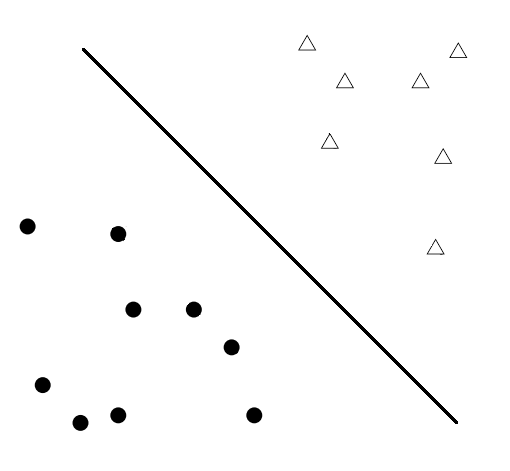
\includegraphics[scale=0.5]{hinh/SVM1.png}
\caption{Minh họa mô hình phân loại dữ liệu có nhãn}
\label{fig:dataclassify}
\end{figure}
\pagebreak
Mô hình SVM chuẩn là một mô hình học máy có giám sát sử dụng thuật toán phân loại nhị phân. SVM nhận đầu vào là một tập dữ liệu biết trước nhãn của mỗi phần tử thuộc tập dữ liệu đó. Ví dụ như ở hình~\ref{fig:dataclassify}, tập dữ liệu đầu vào gồm tập hợp các điểm biết trước phân lớp (hình tam giác, hình tròn). Nhiệm vụ của SVM là xây dựng một đường phân cách tuyến tính chia tập dữ liệu thành hai nhóm điểm thuộc hai lớp khác nhau, sao cho khi có một điểm mới xuất hiện chưa biết trước nhãn, từ vị trí của điểm này so với đường phân cách có thể dự đoán điểm mới thuộc nhóm phân lớp nào. Để giải quyết bài toán này, mô hình SVM sử dụng giải thuật tối ưu hóa khoảng cách giữa đường phân chia tuyến tính đến điểm dữ liệu gần nhất ở cả hai lớp.
\subsubsection*{Giải thuật tối ưu hóa khoảng cách}
\begin{figure}[h] \centering
    \begin{subfigure}[b]{0.325\textwidth}    \centering
        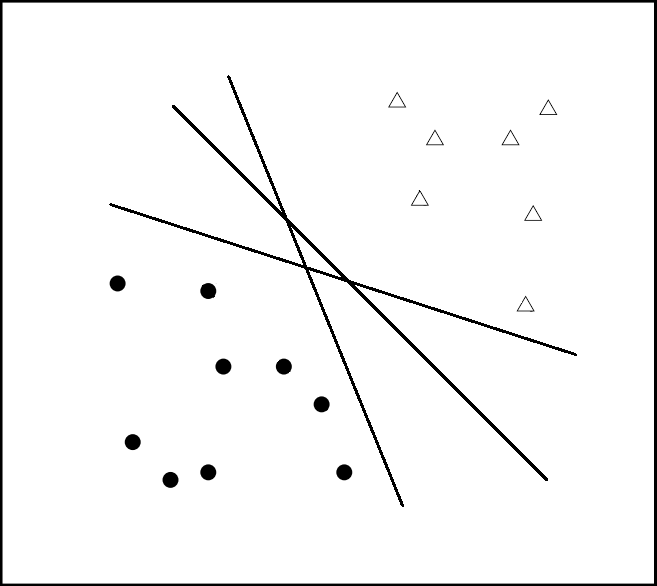
\includegraphics[width=\textwidth]{hinh/SVM2.png}
        \caption{ }
        \label{fig:svm1}
    \end{subfigure}
    \begin{subfigure}[b]{0.325\textwidth}    \centering
        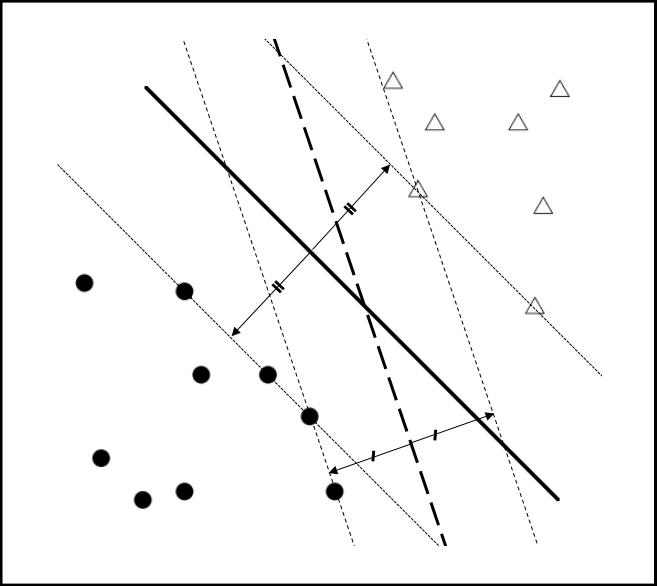
\includegraphics[width=\textwidth]{hinh/SVM3.png}
        \caption{ }
        \label{fig:svm2}
    \end{subfigure}
    \begin{subfigure}[b]{0.325\textwidth}    \centering
        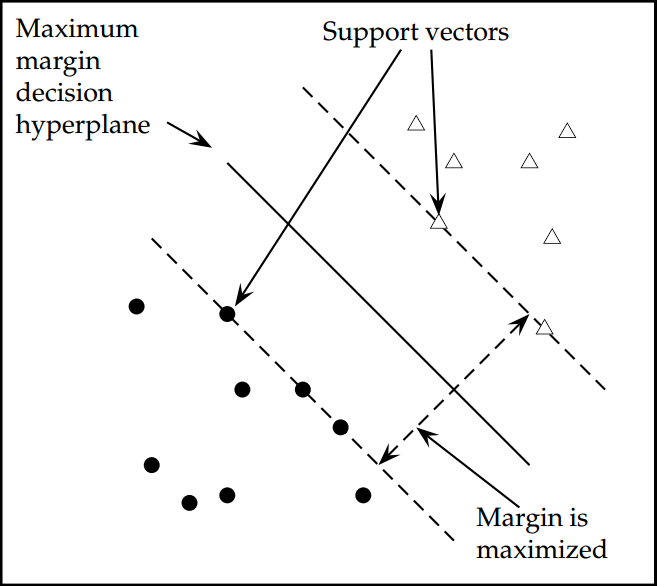
\includegraphics[width=\textwidth]{hinh/SVM4.png}
        \caption{ }
        \label{fig:svm3}
    \end{subfigure}
    \caption[Caption for LOF]{Minh họa giải thuật tối ưu hóa khoảng cách của mô hình SVM \cite{manning2009anintroduction}}
    \label{fig:svm}
\end{figure}
Với không gian dữ liệu tương đối đơn giản như hình~\ref{fig:svm1}, vấn đề đặt ra là có vô số đường tuyến tính có khả năng phân chia tập dữ liệu thành hai lớp phân biệt. Trong tập hợp các đường phân cách này, ta cần lựa chọn một đường tối ưu để tăng hiệu quả phân loại và giảm nhiễu cho tập dữ liệu bằng giải thuật tối ưu hóa khoảng cách của SVM.\\

Đầu tiên, đường phân cách cần nằm cách đều hai nhóm phân loại để đảm bảo xác suất phân loại điểm mới công bằng cho cả hai lớp (hình~\ref{fig:svm2}). Điều này có nghĩa là khoảng cách \textit{D} từ đường phân cách đến điểm gần nhất ở cả hai lớp  phải bằng nhau. Tuy nhiên, số lượng đường tuyến tính đảm bảo yêu cầu trên là vô số. Lúc này ta quan tâm đến độ lớn của \textit{D}: nếu \textit{D} nhỏ, xác suất phân loại sai sẽ cao hơn do sai số của dữ liệu đầu vào trên thực tế. Vì vậy mô hình SVM chọn đường phân loại có khoảng cách lớn nhất đến điểm gần nhất ở cả hai lớp (hình~\ref{fig:svm3}). Các điểm dữ liệu thuộc hai lớp có vị trí gần nhất với đường thẳng phân loại gọi là \textit{support vector}.

\subsubsection*{Kĩ thuật Kernel}
Dựa vào đặc trưng về vị trí điểm dữ liệu, tập dữ liệu đầu vào có thể được chia làm hai loại:
\begin{itemize}
\item[•] Khả phân cách tuyến tính: tồn tại ít nhất một đường thẳng thuộc không gian dữ liệu có thể phân chia tập dữ liệu xác định thành hai nhóm có nhãn khác nhau như hình~\ref{fig:dataclassify}.
\item[•] Không khả phân cách tuyến tính: không tồn tại đường thẳng thuộc không gian tập dữ liệu có khả năng chia các điểm dữ liệu thành hai nhóm có nhãn khác nhau. Lúc này bài toán trở thành phân loại phi tuyến.
\end{itemize}
Trong trường hợp dữ liệu đầu vào không khả phân cách tuyến tính, cách giải quyết đầu tiên là biến đổi không gian dữ liệu trở thành khả phân cách tuyến tính. Nói cách khác, ta cần tìm một hàm ánh xạ sao cho với không gian dữ liệu sau khi ánh xạ tồn tại ít nhất một đường thẳng hoặc mặt phẳng tuyến tính có thể phân loại dữ liệu thành hai lớp. Để làm việc này ta có thể chỉnh sửa các đặc trưng của dữ liệu, hoặc suy diễn đặc trưng mới trên cơ sở những đặc trưng có sẵn. Ngoài ra, ta cũng có thể ánh xạ các điểm dữ liệu vào không gian có số chiều lớn hơn sao cho trong không gian đó có ít nhất một đường thẳng hay mặt phẳng tuyến tính có thể giúp phân loại các điểm dữ liệu (hình~\ref{fig:axkernel}). Hàm ánh xạ thường không cố định và được lựa chọn tùy theo đặc tính của dữ liệu và tính chất bài toán.
\begin{figure}[h]
\centering
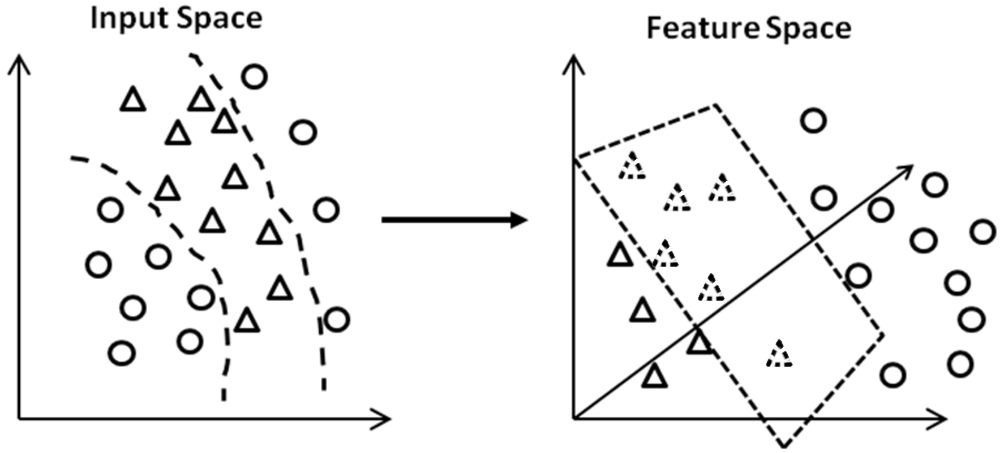
\includegraphics[scale=0.3]{hinh/kernel.png}
\caption[Caption for LOF]{Minh họa ánh xạ tập dữ liệu không khả phân cách tuyến tính \footnotemark}
\label{fig:axkernel}
\end{figure}
\footnotetext{Tham khảo Figure 7 của \cite{pei2012using}}
\subsubsection*{Phương pháp soft-margin}
Trên thực tế, sai số của dữ liệu đầu vào là một trong những nguyên nhân dẫn đến bài toán phân loại phi tuyến. Trong trường hợp này, phương pháp \textit{soft-margin} thường được sử dụng để cải thiện giải thuật tối ưu hóa khoảng cách (hình~\ref{fig:softmargin}). Phương pháp này cho phép tồn tại một số điểm được phân chia sai lớp với một giới hạn sai số nhất định (gọi là độ lỗi).
\begin{figure}[h]
\centering
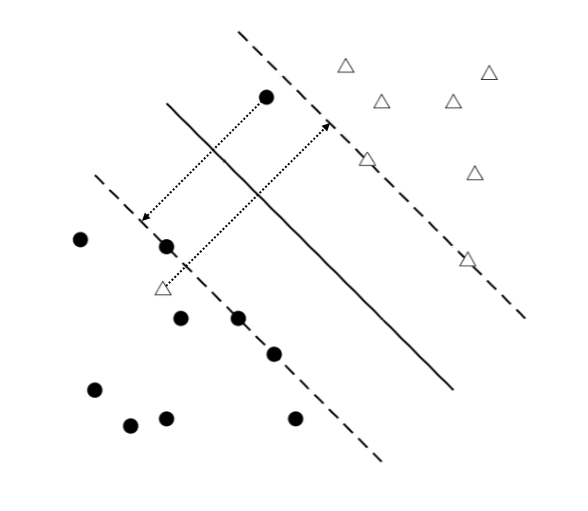
\includegraphics[scale=0.45]{hinh/SVM5.png}
\caption{Minh họa phương pháp soft-margin}
\label{fig:softmargin}
\end{figure}
\subsubsection*{Bài toán phân loại đa lớp}
Mô hình SVM dạng chuẩn như trên chỉ giúp phân loại dữ liệu thành hai lớp. Trong khi đó, bài toán thực tế đòi hỏi số lượng lớp phân loại đầu ra thường lớn hơn 2. Ví dụ như bài toán phân tích cảm xúc trên văn bản y khoa yêu cầu phân loại cảm xúc thành 3 lớp: \tichcuc, \tieucuc và \trungtinh. Lúc này cần áp dụng một hoặc kết hợp một số phương pháp phân loại đa lớp sử dụng mô hình SVM như OvA (One-vesus-All), OvO (One-against-one), DDAG (Decision Directed Acyclic Graph).
\begin{table}[H] \centering
\caption{Minh họa phương pháp phân loại OvA cho bài toán phân tích cảm xúc trong bệnh án điện tử}
\begin{tabular}{ | P{0.2\textwidth} | P{0.2\textwidth} | P{0.2\textwidth} | P{0.2\textwidth} | }
\hline 
\textbf{Bộ phân loại} & \textbf{\tichcuc}& \textbf{\tieucuc} & \textbf{\trungtinh} \\ 
\hline 
\textbf{SVM\textsubscript{1}} & O & X & X \\ 
\hline 
\textbf{SVM\textsubscript{2}} & X & O & X \\ 
\hline 
\textbf{SVM\textsubscript{3}} & X & X & O \\ 
\hline 
\end{tabular}
\label{tab:svmclass} 
\end{table}
Bảng~\ref{tab:svmclass} minh họa phương pháp phân loại OvA: kết hợp nhiều mô hình SVM để phân loại dữ liệu. Trong đó, mỗi SVM giúp phân loại một lớp dữ liệu tương ứng với các lớp khác. Cụ thể với bài toán phân tích cảm xúc trong văn bản y khoa đã đề cập, ta cần ba mô hình SVM: SVM\textsubscript{1} phân loại dữ liệu thành lớp \tichcuc với lớp \textit{Không tích cực} (bao gồm \tieucuc và \trungtinh), SVM\textsubscript{2} phân loại dữ liệu thành lớp \tieucuc với lớp \textit{Không tiêu cực} (bao gồm \tichcuc và \trungtinh), và tương tự với SVM\textsubscript{3}. Khi xuất hiện một điểm dữ liệu mới, dữ liệu đó sẽ được phân loại qua tất cả những lớp SVM đã được xây dựng.

\subsection{Phương pháp đánh giá độ đồng nhất Cohen's kappa}
Hệ số \term{Cohen's kappa}, gọi tắt là \term{kappa}, ký hiệu $\kappa$, là hệ số đánh giá mức độ đồng ý của 2 ý kiến đánh giá trên cùng 1 tập các đối tượng được đánh giá. Trong nghiên cứu này, chúng tôi sử dụng $\kappa$ để đánh giá mức độ đồng ý của 2 người đánh nhãn trên tập dữ liệu. Phương pháp này được đánh giá cao bởi vì $\kappa$ có xem xét đến xác xuất ngẫu nhiên xảy ra sự đồng ý giữa 2 ý kiến đánh giá.\\

Phương pháp hệ số \term{kappa} có 3 phiên bản:
\begin{itemize}
\item[•] Phiên bản gốc do Jacob Cohen giới thiệu năm 1960, thường được gọi là \term{Cohen's kappa}. Trong nghiên cứu này, chúng tôi sử dụng phiên bản gốc.
\item[•] Phiên bản \term{kappa} có trọng số, giúp xét đến cả tỉ lệ không đồng ý.
\item[•] Phiên bản \term{Fleiss' kappa} có thể đo độ đồng nhất với số lượng người đánh nhãn không giới hạn, trong khi phiên bản gốc chỉ có thể đánh giá khi có đúng 2 người đánh nhãn.
\end{itemize}
Mỗi người đánh nhãn được yêu cầu phân loại mỗi câu thuộc vào 1 trong 3 loại: \tichcuc, \tieucuc hoặc \trungtinh. Từ đó, các câu đã đánh nhãn được thống kê như Bảng \ref{table:kappa}.
\begin{table}[H]
\caption{Thống kê các câu được đánh nhãn} \label{table:kappa}
\begin{tabular}{|m{2cm}|l|l|l|l|l|}
\hline
	& \multicolumn{5}{c|}{\textbf{Người đánh nhãn 1}}                                                                \\ \hline
\multirow{5}{2cm}{\textbf{Người đánh nhãn 2}} & \textbf{}           & \textbf{Tích cực} & \textbf{Tiêu cực} & \textbf{Trung tính} & \textbf{Tổng cộng}         \\ \cline{2-6} 
                                            & \textbf{Tích cực}   & $p_{11}$          & $p_{12}$          & $p_{13}$            & $p_{1a}$                      \\ \cline{2-6} 
                                            & \textbf{Tiêu cực}   & $p_{21}$          & $p_{22}$          & $p_{23}$            & $p_{2a}$                      \\ \cline{2-6} 
                                            & \textbf{Trung tính} & $p_{31}$          & $p_{32}$          & $p_{33}$            & $p_{3a}$                      \\ \cline{2-6} 
                                            & \textbf{Tổng cộng}  & $p_{1b}$             & $p_{2b}$             & $p_{3b}$               & $p$ (Tổng số câu) \\ \hline
\end{tabular}
\end{table}
Hệ số kappa được tính bởi công thức:
$$\kappa = \dfrac{p_o - p_e}{1 - p_e} = 1 - \dfrac{1-p_o}{1-p_e}$$
Trong đó:
\begin{itemize}
\item[•] $p_o$ là tỉ lệ đồng ý tương đối giữa 2 người đánh nhãn. $p_o = \dfrac{p_{11}+p_{22}+p_{33}}{p}$
\item[•] $p_e$ là giả thiết xác suất 2 người đánh nhãn đồng ý ngẫu nhiên. Xét các câu được đánh nhãn \tichcuc, xác suất để người thứ nhất đánh 1 câu thuộc nhãn \tichcuc là $p_{1b}/p$, xác suất để người thú 2 đánh 1 câu thuộc nhãn \tieucuc là $p_{1a}/p$, do đó, xác xuất ngẫu nhiên 2 người cùng đánh 1 câu thuộc nhãn \tichcuc là: 
$$\dfrac{p_{1b}}{p} * \dfrac{p_{1a}}{p}$$
Từ đó, $p_e$ là tổng xác suất ngẫu nhiên 2 người cùng đánh 1 câu thuộc nhãn \tichcuc, \tieucuc, \trungtinh:
$$p_e = \frac{p_{1a}}{p}*\frac{p_{1b}}{p} + \frac{p_{2a}}{p}*\frac{p_{2b}}{p} + \frac{p_{3a}}{p}*\frac{p_{3b}}{p}$$
\end{itemize}

Nếu 2 người đánh nhãn hoàn toàn đồng ý với nhau, $p_o=1$ và $p_e = 0$, suy ra $\kappa=1$. Ngược lại, $\kappa<0$ nếu tỉ lệ đồng ý giữa 2 người đánh nhãn thấp hơn cả xác xuất đồng ý ngẫu nhiên. Theo nghiên cứu \cite{Viera2005}, độ đồng nhất giữa 2 người đánh nhãn được đánh giá như Bảng \ref{table:thang-do-kappa}
\begin{table}[H]
\centering
\caption{Thang đo đánh giá độ đồng nhất dựa trên giá trị $\kappa$} \label{table:thang-do-kappa}
\begin{tabular}{|c|l|}
\hline
Giá trị & Mức độ đồng nhất \\ \hline
$\kappa<0$ & Thấp hơn xác xuất đồng ý ngẫu nhiên \\ \hline
$0.1<\kappa<0.2$ & Hơi đồng ý (\term{slight}) \\ \hline
$0.21<\kappa<0.40$ & Mức độ khá (\term{fair}) \\ \hline
$0.41<\kappa<0.60$ & Mức độ vừa phải (\term{moderate}) \\ \hline
$0.61<\kappa<0.80$ & Mức độ tốt (\term{substantial}) \\ \hline
$0.81<\kappa<0.99$ & Mức độ gần như hoàn hảo (\term{almost perfect}) \\ \hline
\end{tabular}
\end{table}

\subsection{Các thư viện và công cụ hỗ trợ}
\subsubsection*{Thư viện UMLS}
UMLS (\term{Unified Medical Language System}) là hệ thống từ vựng y sinh do Thư viện Y khoa Quốc gia Hoa Kỳ xây dựng từ năm 1986 bao gồm tập dữ liệu lớn các thông tin y khoa đã được chuẩn hóa và những công cụ hỗ trợ tương tác với hệ thống máy tính. Tính đến năm 2004, bộ từ điển UMLS tích hợp hơn 2 triệu tên gọi cho khoảng 900.000 khái niệm y sinh và khoảng 12 triệu tên gọi cho quan hệ giữa các khái niệm này \cite{Bodenreider2004}. Hiện nay UMLS vẫn liên tục được câp nhật và cho phép sử dụng miễn phí phục vụ mục đích nghiên cứu khoa học.\\

Hệ thống UMLS chứa 3 thành phần chính:
\begin{itemize}
\item Kho dữ liệu Metathesaurus\footnote{https://www.nlm.nih.gov/research/umls/knowledge\_sources/metathesaurus/}: là bộ từ điển y sinh lớn chứa các thông tin như mã số, ngữ nghĩa của các loại từ vựng, thuật ngữ y học và nhãn liên kết giữa các từ vựng khác nhau có cùng khái niệm. Metathesaurus là thành phần lớn nhất của UMLS, được tích hợp từ mạng ngữ nghĩa và các công cụ xử lý ngôn ngữ tự nhiên trong UMLS. Kho dữ liệu Metathesaurus bao gồm nhiều thư viện y khoa được sử dụng phổ biến như MeSH\footnote{https://www.ncbi.nlm.nih.gov/mesh}, SNOMED CT\footnote{https://www.nlm.nih.gov/healthit/snomedct/},...
\item Mạng ngữ nghĩa (\term{Semantic Network}) chứa danh mục các loại ngữ nghĩa và mối quan hệ giữa chúng.
\item Công cụ từ vựng (\term{SPECIALIST Lexicon and Lexical Tools}) bao gồm các công cụ xử lý ngôn ngữ tự nhiên được dùng để tích hợp Metathesaurus.
\end{itemize}

\subsubsection*{Công cụ MetaMap}
MetaMap là công cụ hỗ trợ việc nhận dạng các khái niệm trong bộ từ điển UMLS-Metathesaurus từ văn bản y khoa. MetaMap nhận dữ liệu đầu vào là văn bản phi cấu trúc, thuần ngôn ngữ tự nhiên như các loại báo cáo y khoa, văn bản khám lâm sàng,... Sau quá trình xử lý, đầu ra của MetaMap là văn bản có cấu trúc - chủ yếu ở định dạng XML hoặc một số định dạng khác như MMO, HR - chứa các khái niệm nhận dạng được trong kho dữ liệu Metathesaurus từ văn bản đầu vào. Kiến trúc tổng quát của MetaMap được mô tả như hình~\ref{fig:kientrucmetamap}.\\

\begin{figure}[h]
\centering
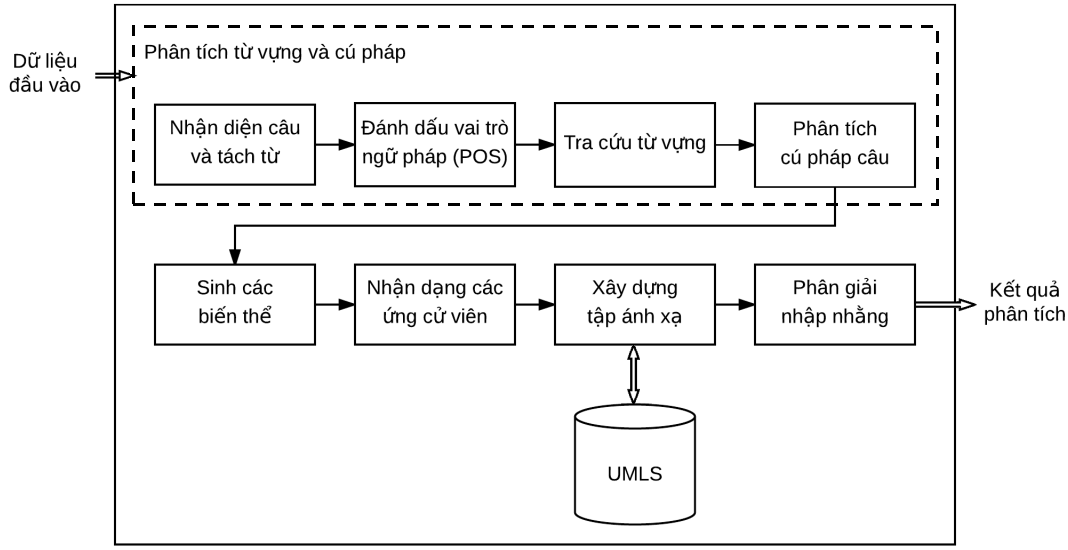
\includegraphics[scale=0.52]{../hinh/KienTrucMetamap.png}
\caption{Kiến trúc tổng quát của MetaMap \cite{Aronson2010}} \label{fig:kientrucmetamap}
\end{figure}

Quá trình xử lý của MetaMap có thể được tóm tắt qua 2 bước:
\begin{enumerate}
\item Phân tích từ vựng và cú pháp: dữ liệu đầu vào được áp dụng các tác vụ xử lý ngôn ngữ tự nhiên cơ bản như tách câu, tách từ, xác định từ loại, tra cứu từ vựng dùng công cụ từ vựng của UMLS và phân tích cú pháp câu. Sau những tác vụ này, kết quả thu được là tập hợp các cụm từ (\term{phrase}) được xác định từ văn bản đầu vào.
\item Phân tích chuyên sâu: ứng với mỗi cụm từ đã tìm được, MetaMap tiến hành tìm tất cả những biến thể của cụm, xác định các ứng cử viên (candidate) từ các khái niệm trong UMLS khớp với các biến thể được sinh ra và đánh giá độ tin cậy của từng ứng viên. Kết quả thu được là tập hợp các cụm đã có từ bước 1, và thông tin các ứng cử viên tương ứng.
\end{enumerate}

Ví dụ với đầu vào là câu: \myquote{He denied chest pain, shortness of breath or cough.} Kết quả sau khi phân tích của MetaMap trả về như hình~\ref{fig:metamapsample}. Các ứng cử viên được gọi tên là Meta Mapping. Câu văn được tách thành các cụm: \myquote{He}, \myquote{denied}, \myquote{chest pain}, \myquote{shortness of breath}, \myquote{or}, \myquote{cough}. Trong đó:
\begin{itemize}
\item Các cụm \myquote{He}, \myquote{or} không có Meta Mapping do không tìm được ứng cử viên nào.
\item Cụm \myquote{denied} có 2 Meta Mapping cùng số điểm tin cậy (1000), tương ứng với 2 khái niệm trong UMLS Metathesaurus với 2 mã định danh CUI (\term{Concept Unique Identifier}) là C0332319 và C2700401, kèm theo là định nghĩa, mô tả và nhóm của khái niệm đó. Với cụm \myquote{denied}, MetaMap xác định được 2 nhóm là Khái niệm định tính (\term{Qualitative Concept}) và Hành động (\term{Activity}).
\item Tương tự như cụm \myquote{denied}, các cụm \myquote{chest pain}, \myquote{shortness of breath}, \myquote{chest pain} cũng có 2 Meta Mapping với đầy đủ mã số CUI, định nghĩa, mô tả và nhóm của từng khái niệm.
\end{itemize}

\begin{figure}[h]
\centering
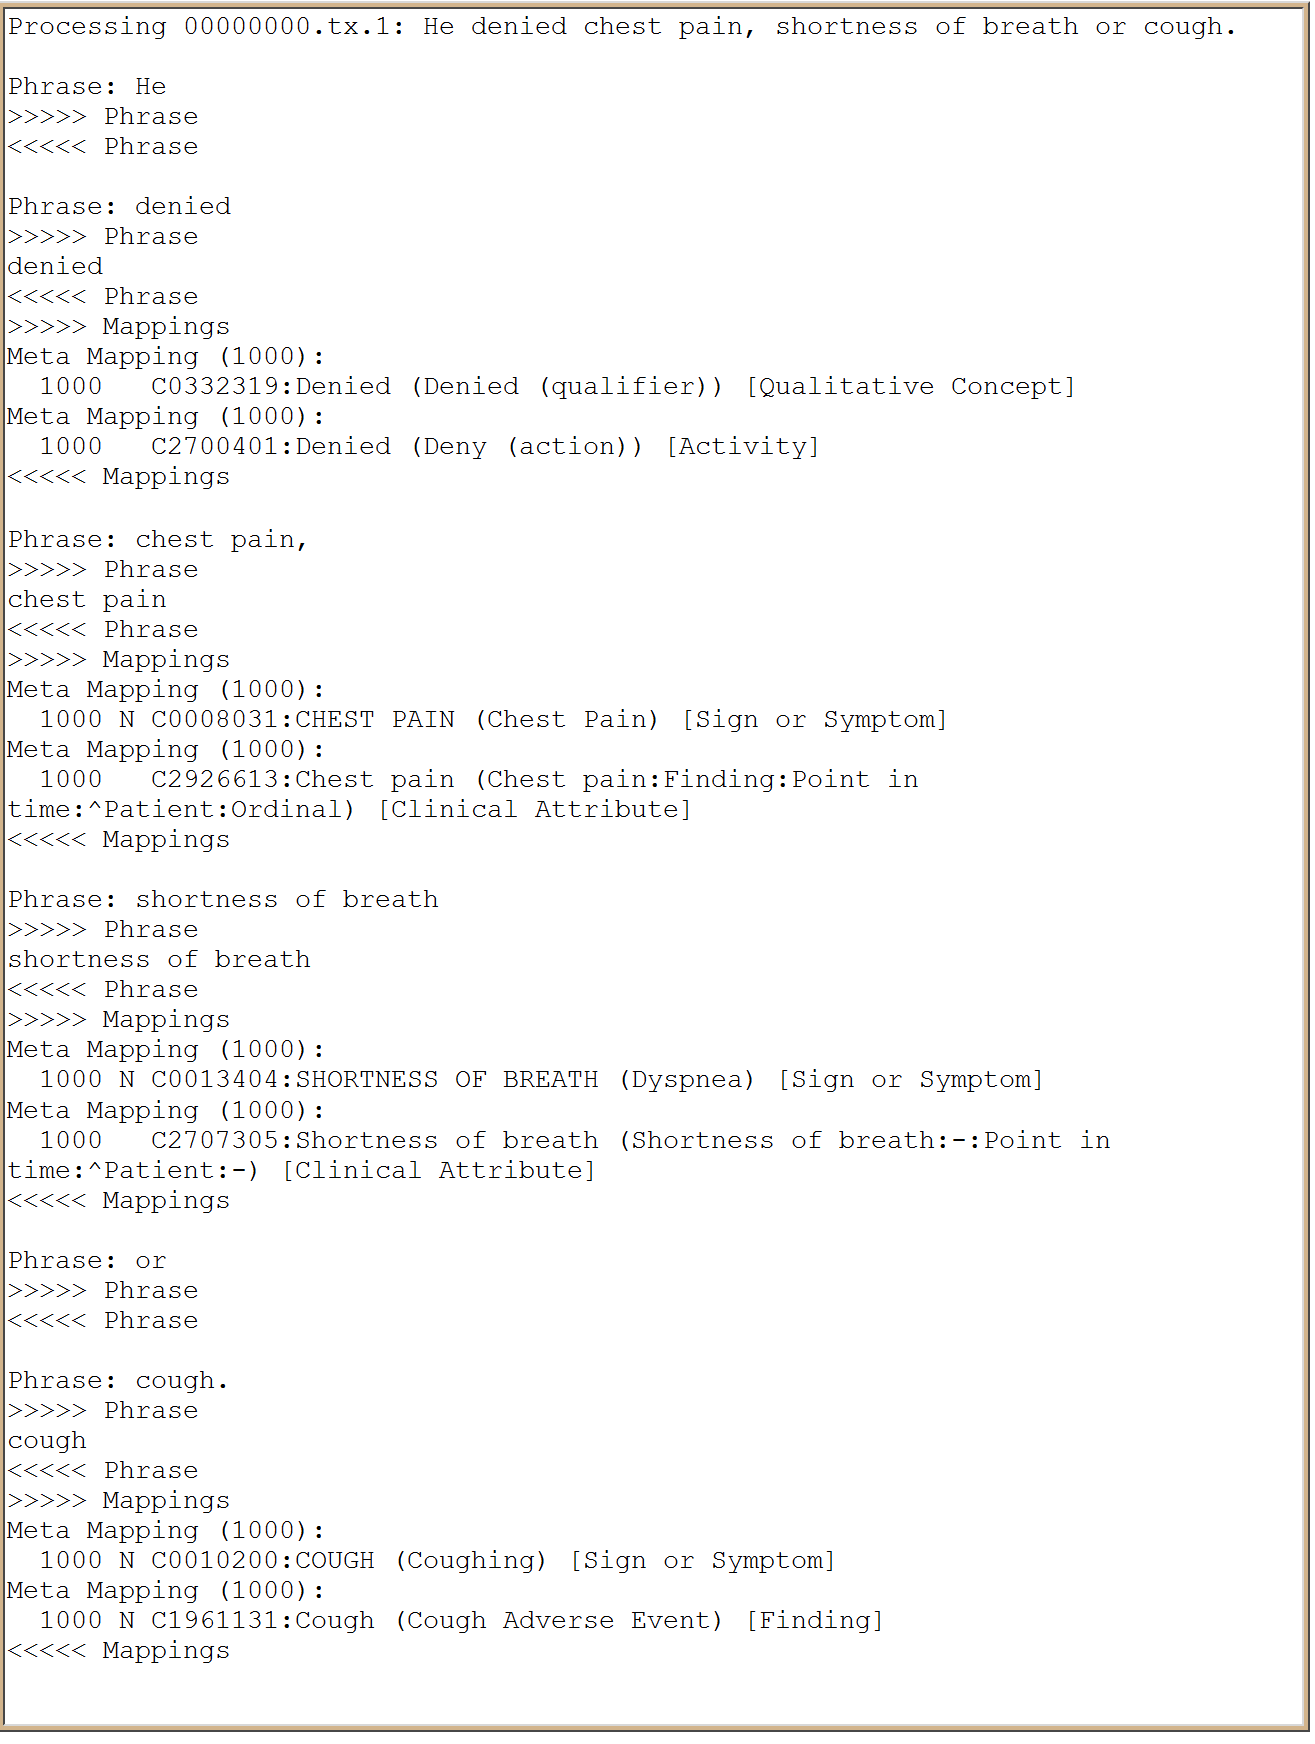
\includegraphics[scale=0.35]{../hinh/metamapsample.png}
\caption{Ví dụ kết quả chạy MetaMap}
\label{fig:metamapsample}
\end{figure}

Không chỉ xác định nhóm ngữ nghĩa của các khái niệm, MetaMap còn hỗ trợ phân tích các yếu tố phủ định có trong dữ liệu đầu vào. Khi chọn bộ lọc \myquote{-negex}, kết quả phân tích sẽ thêm ký tự \myquote{N} vào trước khái niệm bị phủ định. Ví dụ như hình~\ref{fig:metamapsample}, cụm \myquote{chest pain} có 1 Meta Mapping với mã khái niệm C0008031, thuộc nhóm Dấu hiện hoặc triệu chứng (\term{Sign or Symptom}) bị phủ định.
